\label{chapter1}

In recent years, the field of soft robotics has received a substantial increase of interest \cite{iida2011soft},\cite{walker2020soft}, \cite{bao2018soft}. Soft robots have a vast domain in which they can be applied. This includes the medical field \cite{sitti2018miniature} \cite{ashuri2020biomedical}, where soft robots have potential applications in artificial muscles, prosthetic devices, stents and surgical instruments. They can also be used to explore places that are hard to reach for human beings. This includes offshore operation and deep-sea exploration \cite{aracri2021soft}, such as the soft robot exploring the depths of the Mariana trench \cite{laschi2021soft}. Other applications are in the field of industrial automation, where they can support human operators in manipulating objects \cite{george2018control}, \cite{grissom2006design}. A variety of experimental soft robots are displayed in Figure \ref{fig1:softexample}. 



\begin{figure}[H]       
    \centering
    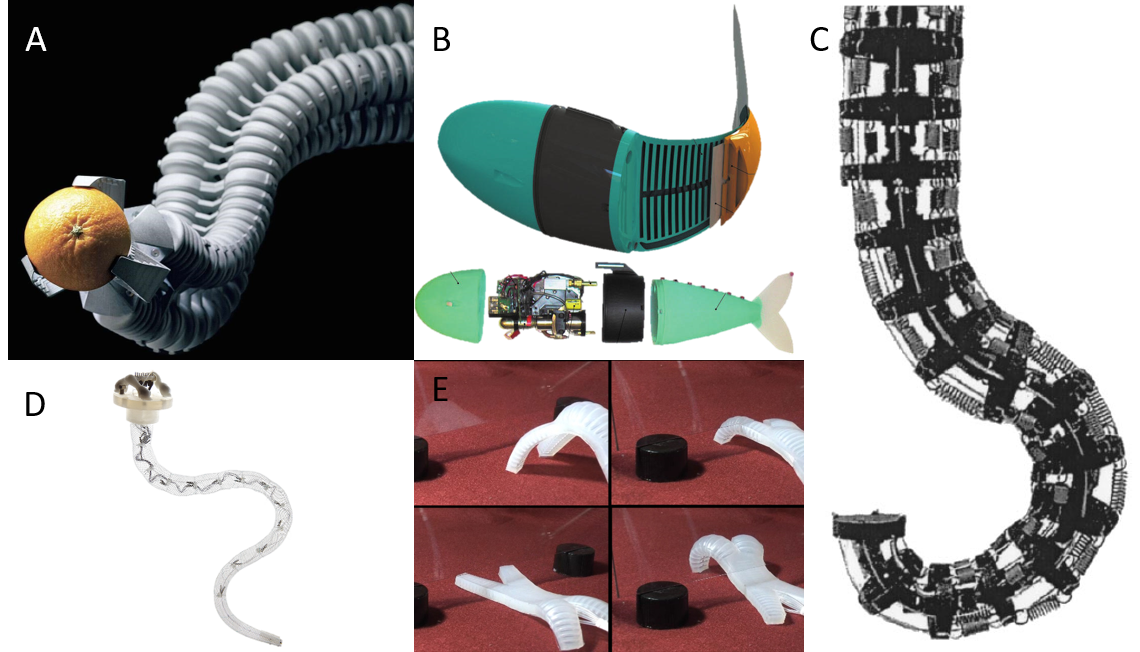
\includegraphics[width = \textwidth]{Figures/Chapter1/robotexamples.png}
    \caption{\textbf{A}: Bionic Handling Assistant inspired by the trunk of an elephant \cite{BHA}. \textbf{B}: Bio-inspired soft robot replicating movement of a fish \cite{marchese2014}. \textbf{C}: Elephant’s Trunk Manipulator \cite{hannan2003kinematics}. \textbf{D}: Bio-inspired soft octopus tentacle \cite{laschi2012soft}. \textbf{E}: Pneumatically actuated starfish like soft robot \cite{shepherd2011multigait}.}
    \label{fig1:softexample}
\end{figure}


The foundation of soft robotic design is often found in nature and includes inspiration for material choice, locomotion, and morphology. As their name already suggests, soft robots are made from soft and flexible materials. Their inherently dexterous structure allows soft robots to move around obstacles. This makes soft robots robust and very applicable in constantly changing environments. A few examples of bio-inspired soft robots include emulated trunks \cite{hannan2003kinematics} inspired by the proboscis of an elephant, robots based on the arm of octopus \cite{wang2013visual}, and robots that replicate the movement of fish \cite{marchese2014}, Figure \ref{fig1:softexample}. 


\subsection*{Soft robot manipulators vs. traditional manipulators }

In this thesis, we focus on soft robots designed for manipulating objects. These robots reshape the idea of using robots for industrial processes. Currently, rigid robots dominate the field of industrial automation, as they excel in accuracy, repeatability and load capacity. However, these traditional robots tend to be unsafe when operating in human-centred environments. Classic robots are composed of rigid materials and accelerate to high velocities, which could create an unsafe environment for human operators. Additionally, these robots have limited degrees of freedom, making it harder to avoid obstacles. To evade the risk of potential harm, and create more dexterous robots, innovative soft robotic manipulators are designed. As they are made from soft materials they are inherently safer to operate around humans. However, due to their flexible nature, they behave differently compared to traditional robots. To gain a better understanding of soft robotic manipulators, we will draw parallels and mention differences between these type of soft robots and traditional robots: i) material, ii) actuation, iii) sensing.


First, a classification between both can be made based on the compliance of their underlying materials \cite{Bionics2008}. Generally, classic robots are made of rigid metal beams, whereas soft robots are made from soft polymer materials. The building materials of the robot largely determine the kinematic redundancy of the robot. Since soft robots are composed of materials with an extremely low Young's modulus, they can sustain large (and possibly non-linear) deformation during normal operation. As a result of this compliance, gravity and payload cause a distributed deformation throughout the entire system. This gives the robot theoretically an infinite amount of degrees of freedom. This makes controlling these robots more challenging when compared to traditional robots, as the latter has a fixed amount of degrees of freedom.

Secondly, actuation is another major difference between the two robot types. Whereas traditional robots are generally electro-mechanically actuated, soft robots can be actuated with a wide range of actuation methods, which includes pneumatics, hydraulics, thermal and even chemical \cite{BHA},\cite{marchese2014},\cite{kang2019programmable},\cite{shepherd2013using}. Rigid robots are often linked by rotatory or prismatic joints, where its design allows to include the actuator inside the robot's casting or joint. The actuators of soft robots are often located externally, as their design simply does not allow to integrate them. Most soft robot manipulators are actuated pneumatically or by using variable-length tendons \cite{Rus2015}. A well-known example of a pneumatically actuated soft robot is the Bionic Handling Assistant (BHA) by Festo, as shown in Figure (\ref{fig1:softexample}). These type of soft robots have inflatable channels that cause deformation when applying pressure. An example of a tendon driven robot is the elephant trunk's robot \cite{cieslak1999elephant} (Figure \ref{fig1:softexample}). This manipulator consists of eight elastic segments linked together by coil springs. Each segment is controlled by two pairs of strings. Servo or linear actuators are used to wind and unwind the strings, with that controlling the movement of the robot. Both actuation methods introduce additional dynamics that largely affect the performance of the entire control system. 

Thirdly, conventional sensing mechanisms can often not be applied to soft robots. For hard robots, their joint design allows incorporating encoders to measure rotation and other sensory devices. Since the forward kinematics, given rigid joints and links, can be computed through trigonometry, position sensing is relatively easy. For soft robots, the compliant and lightweight nature often prevents the integration of conventional sensors, such as encoders, strain gauges and inertial measurement units (IMU's) \cite{Rus2015}, \cite{Lee2017}. Alternative sensory techniques are often needed. These methods include for instance optical sensors and stretch sensors based on macrobend fibres \cite{Sareh2015}.

\subsection*{Control strategies}
The aforementioned discussed the contrast between rigid robots and soft robots. It showed that soft robot manipulators distinct themselves from traditional robots on three fronts. Their inherent soft body leads to a theoretical infinite degree system. The actuation of soft robots introduces additional dynamics caused by the actuators. Furthermore, the conventional sensory mechanisms can often not be applied to soft robots, and therefore demand more complex sensory devices. These factors all affect the way soft robots can be controlled. Recent literature often tries to convey readily available control theories and apply those to soft robotics.

The work of Thuruthel et al. (2018) \cite{george2018control} presents an overview of recent findings in soft robotic control for pneumatically actuated and tendon-driven soft robots. In this work, three control approaches are distinguished, namely model-free, hybrid and model-based control. A model-free control strategy does not use kinematic or dynamic description in its control approach. Instead, it exploits learning-based algorithms to dynamically control the robotic system. Hybrid controllers combine learning or empirical elements with a model-based approach. The model-based controllers rely on an analytical description of the robotic system. Furthermore, for each control approach, a sub-division between kinematic and dynamic control is made. Here, kinematic control is defined as a zero-order input-output relation. A change in input is directly observed in output, therefore this approach is lower-level compared to dynamic control. For the latter, the configuration space and/or task space variables' velocities are used in the control algorithm. 


Research conducted on the Bionic Handling Assistant, as shown in Figure \ref{fig1:softexample}, demonstrates that multiple control methods can be applied to the same robot. A model-free control approach was implemented in \cite{rolf2013efficient}. The inverse kinematics of the robot were obtained through machine learning, instead of model-derivation. Later work shows the implementation of a hybrid controller \cite{reinhart2017hybrid}. In this approach, an inverse kinematic model was used together with a learning model. Previous to this hybrid controller, a model-based controller was proposed by \cite{mahl2014bhakin}. However, this model-based controller only used a kinematic description of the soft robot. This research was followed up by \cite{falkenhahn2016dynamic}, which developed a dynamic controller. In this latter work, the system is controlled with a nonlinear length controller based on feedback linearization. This controller was further supported by linear PD and feedforward control. 

In \cite{wang2013visual} visual servo control is used to control a cable-driven soft robotic manipulator. The manipulator, inspired by an octopus' tentacle, is shaped like a cone. On the outer surface of the soft robot four cables are uniformly distributed. These cables are on one end connected to the tip of the manipulator and on the other side connected to pulleys. By winding and unwinding the cables on the pulleys, the end-effector can be positioned in the task space. A kinematic-based visual servo controller is designed, based on linear PD feedback control with gravity compensation. Position sensing is done by a camera mounted at the tip of the robot, and a fixed feature point. Based on this visual information, a jacobian matrix is estimated, which is used in the kinematic controller.

In \cite{zhang2017visual} also visual servo control was implemented to control a tendon-driven soft robotic manipulator. Again, kinematic control is used for a reference tracking problem. Contrary to the previous research, where a jacobian matrix is estimated, here the jacobian is calculated by running a real-time FEM model parallel. The reference input runs through the FEM model, which outputs a jacobian and expected end-effector position. The jacobian is used in the controller to control the actual manipulator. The FEM model's expected end-effector position and actual end-effector position are used in a second controller to enhance jacobian estimation in the FEM model.

A model-based controller that uses a dynamic model in its control loop is presented in \cite{della2020model}. The robots infinite dimensionality is resolved by regarding the robot being composed of six individual actuatable segments. A piece-wise constant curvature (PCC) approach was used to describe the kinematics of the robotic actuator. For each segment, Denavit-Hartenberg (DH) parameters are used to describe the rigid robot equivalent, which is then used to derive a dynamic model. The proposed controller essentially is a computed torque controller with an additional PD controller. 

\subsection*{Modeling of soft robots}

In the aforementioned work, \cite{della2020model}, the infinite dimensionality of the soft robot is solved by assuming the robot consists of a fixed amount of segments. In this way, the infinite-dimensionality of the system can be approximated by a fixed amount of degrees of freedom. This makes controller design easier. Of course, the reduction of degrees of freedom is at the cost of model accuracy. In the work of \cite{della2020model}, the PCC modelling approach was applied, which is a widely adopted method for describing the configuration of soft robots \cite{ccapproach}. This modelling approach can be applied to soft robots that undergo a very specific deformation. Previous research that used this model include \cite{mahl2014bhakin},\cite{ccapproach},\cite{berkers},\cite{Falkenhahn2015},\cite{runge2017framework}. A schematic drawing of the constant curvature modelling approach is shown in Figure \ref{fig2:ccapproach}. Although our modelling approach distinguishes itself from this methodology, it is important to grasp the basics. 

The constant curvature describes the position of the actuator by three coordinates. Parameter $l$ is the curved length of the actuator measured from the fixed bottom to the tip. Coordinate $\kappa$ expresses the curvature of the actuator. It is assumed that the deformed actuator describes a perfect arc, hence radius $r$ is equal to $\frac{l}{k}$. This allows writing the orientation of the actuator's tip as $\theta = l\kappa$. Lastly, parameter $\phi$ describes the rotation of the actuator relative to the ground. A single constant curvature is not able to describe complex actuator configurations. To this end, multiple of these curves are stacked onto each other, thereby discretizing the actuator. This allows describing more complex configurations. This methodology is used in for instance \cite{Falkenhahn2015}.



\begin{figure}[H]
    \centering
    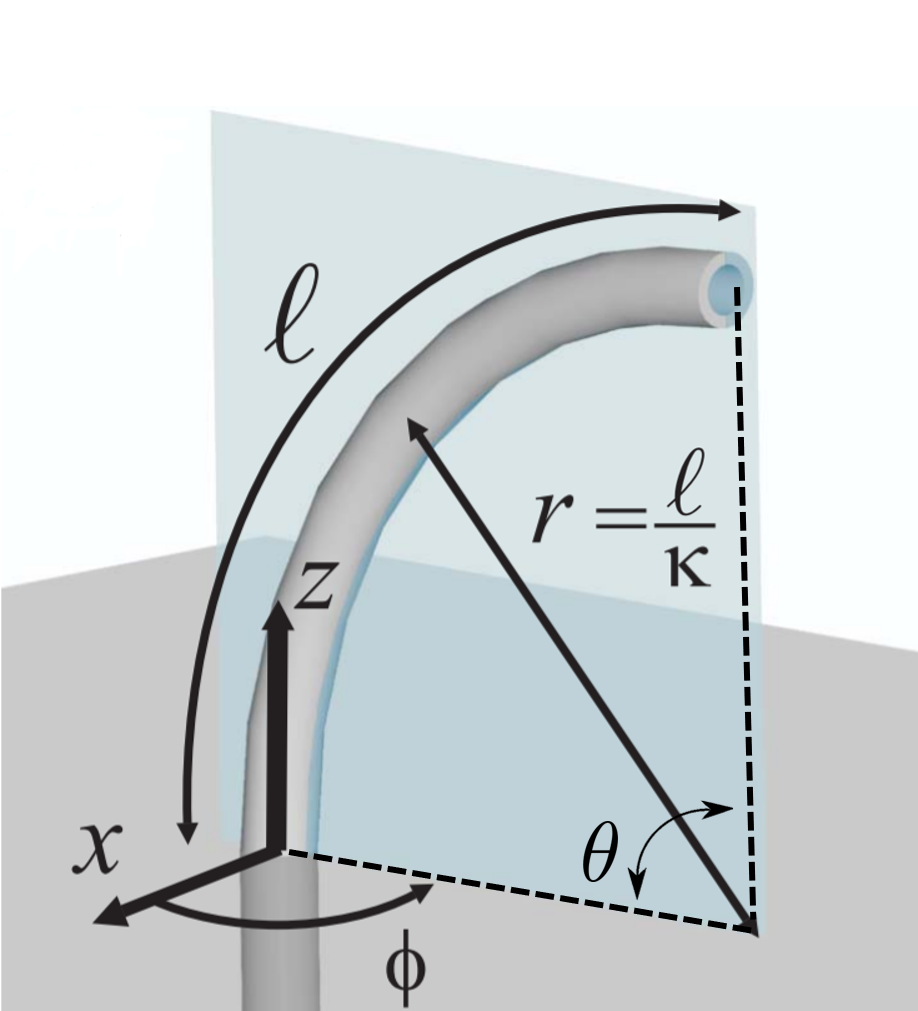
\includegraphics[width = 0.45\textwidth]{Figures/Chapter1/ccapproach2.png}
    \caption{Schematic drawing of the constant curvature model, adapted from \cite{ccapproach}.}
    \label{fig2:ccapproach}
\end{figure}

The PCC approach has some limitations, due to its piece-wise character the actuator configuration is not described by a single continuous function. This makes it harder to find analytical expressions e.g. derivatives. Additionally, this PCC approach only allows assigning material properties to particular points. This makes dynamic models generally less accurate. A method to overcome this problem is using partial differential equations (PDE's) to describe actuator configurations. These PDE's are more suitable for deriving continuum dynamic models. One of these models is the Cosserat beam model which will be exploited in this work. This Cosserat model describes the soft robot configuration as a continuous curve. This continuous curve reflects strains in the backbone of the (deformed) soft robot. These strains can be approximated, hereby reducing the theoretical infinite-dimensional system to a reduced-order form. This dimension reduction allows dynamic model derivation for the soft robot. This dynamic model can then be utilized for model-based control purposes.


\begin{figure}[H]
\begin{minipage}{.5\textwidth}
  \centering
  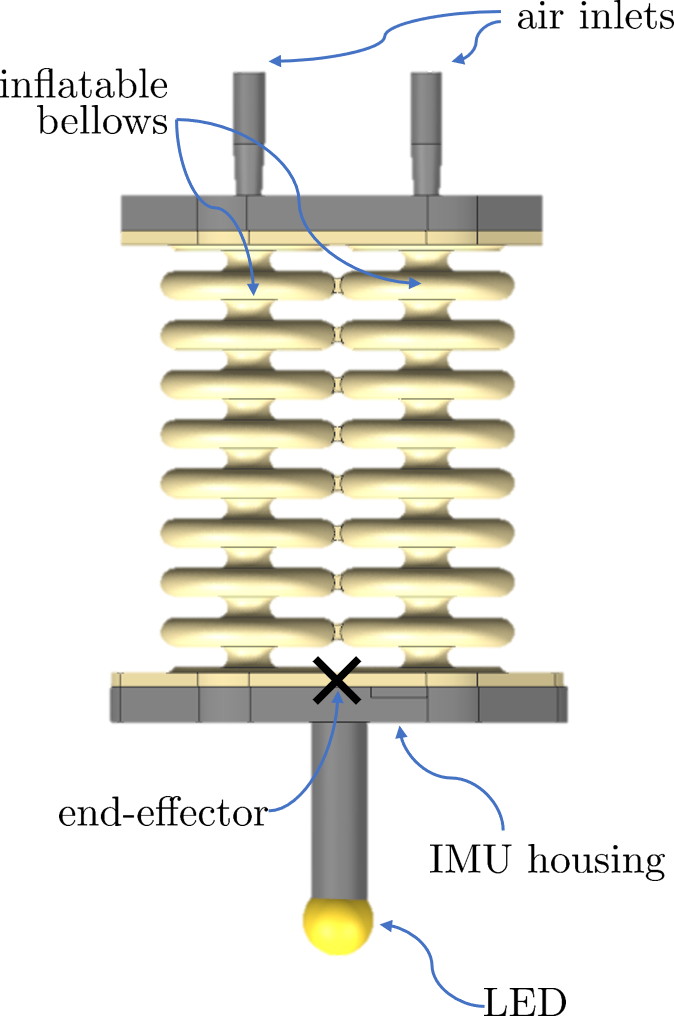
\includegraphics[width = 0.6\linewidth]{Figures/Chapter1/completesetup2.png}
  \caption{Computer rendered image of the soft robot setup }
  \label{fig:test1}
\end{minipage}
\hspace{10pt}
\begin{minipage}{.5\textwidth}
  \centering
  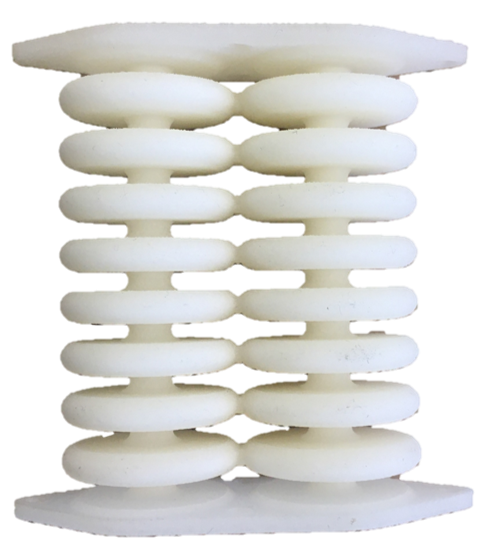
\includegraphics[width =0.6\linewidth]{Figures/Chapter1/actuator.png}
  \vspace{60pt}
  \caption{Planar soft robot, that can change its posture by inflating or deflating the bellows.}
  \label{fig:test2}
\end{minipage}
\end{figure}



\section*{Thesis outline and contribution}

In this work, we study the modelling and control of a planar soft robot as shown in Figure \ref{fig:test2}. This soft actuator has a theoretically infinite amount of degrees of freedom, as it is composed of flexible polymer. Furthermore, it is pneumatically actuated, inducing additional dynamics into the control system, and a major limiting factor on achievable bandwidth. The soft robot consists of two individually inflatable bellows, allowing the robot to extend and curve. Each of the bellows can be inflated using air pumps. The induced rotation can be measured with an inertial measurement unit (IMU), which is mounted at the tip of the actuator. Using optical tracking, an LED marker connected to the tip of the robot can measure the elongation of the robot. The air pumps and sensory devices allow us to design a closed-loop controller, to perform set-point regulation. A schematic layout of the actuator setup is depicted in Figure \ref{fig:test1}.

This work is a continuation of the research of \cite{berkers}, which detailed a length and curvature controller for the planar soft robot. This work uses standard PD and PID control methods to ultimately perform a reference tracking problem. The obtained results are reasonable but do allow for better tracking performance. To enhance the performance of the control system we would like to include model-based information in the control loop. The fundamentals of this research are provided in \cite{Caasenbrood2020}, which developed a framework to model soft robot dynamics. This model is valuable for soft robotic control. Given the system description and previous research conducted on the planar soft robot, the research question that we try to answer is:

\textit{Can we develop a model-based control strategy for a pneumatically actuated, planar soft robot to perform a reference tracking problem?}



To effectively answer the research question we consider the control layout as shown in Figure \ref{fig1:controlarchitecture}. This control setup also shows the structure of this thesis. In Chapter \ref{chap2} a forward kinematic description of the actuator is derived. This allows studying the robot's configuration in 2D-space. Furthermore, it allows us to study the velocity of the actuator as a function of kinematic configuration. The latter allows us to derive a dynamic model of the actuator. Also, a pump model is presented, which allows describing the entire system dynamics in state-space formulation. Once this model is derived, a parameter study is performed in Chapter \ref{chap3}. Here finite element analysis (FEA) is used to capture the non-linear stiffness of the soft robot. Furthermore, experiments are presented which allow determining the pump dynamics. In Chapter \ref{chap4} a model-based controller is proposed. This controller will be tested in simulation, using the dynamic model as derived in Chapter \ref{chap2}. These simulation results, together with experimental verification are presented in Chapter \ref{chap5}.




\begin{figure}[H]
    \centering
    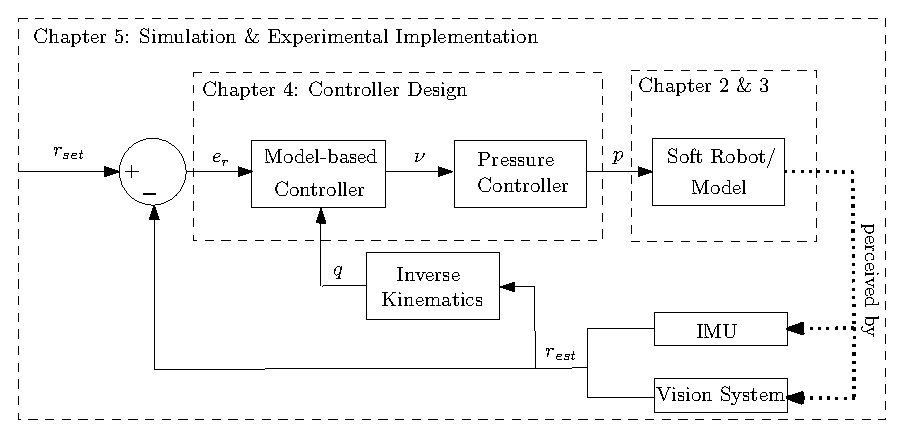
\includegraphics[width = \textwidth]{Figures/Chapter1/controlschemeCompleteGood.eps}
    \caption{Thesis layout and control setup.}
    \label{fig1:controlarchitecture}
\end{figure}


Recapitulating, this thesis comprises the following:


\begin{itemize}
    \item Chapter 2: Development of a non-linear dynamic model
    \item Chapter 3: Modeling of non-linear soft robot stiffness through finite element analysis
    \item Chapter 3: Experimental determination of pump dynamics
    \item Chapter 4: Development of a model-based control law
    \item Chapter 5: Experimental implementation of a model-based controller
\end{itemize}


